\subsection{Закон сохранения энергии и типы орбит}
Для движения тела c массой $m$ в гравитационном  в поле тела 
с массой \linebreak $M\gg m$ со скорость $v$ на расстоянии $r$ от 
гравитационного центра справедливо следующее соотношение: 
\begin{equation}
\frac{m v^2}{2}-\frac{GM m }{r}=E_0,
\end{equation}
где $E_0$ --- постоянная величина, если на тело не действуют
внешние силы кроме силы притяжения к центральному телу, 
равная сумме кинетической и потенциальной энергии тела.

Если $E_0>0$, то траектория тела --- {\itshape гипербола}, 
ветви которой асимптотически приближаются к двум прямым.

Если $E_0=0$, то траектория тела --- {\itshape парабола}. При 
параболической и гиперболический траекториях движение не 
ограничено (инфинитно).

Если $E_0<0$, то траектория тела --- {\itshape эллипс}. При 
эллиптической траектории движение ограничено (финитно).

Параболическая скорость --- минимальная, при которой 
тело покидает центральное тело. Она также называется
{\itshape вторая космическая скорость}. Выражение для нее 
имеет следующий вид:\begin{equation}
v_{2}=\sqrt{\frac{2GM}{r}}
\end{equation}

На Рис. \ref{pic:orbits} представлены примеры возможных траекторий тела 
относительно центрального (точка C). При $v_0 > v_{2}$ --- тело движется 
по гиперболе, при $v_0 = v_{2}$ --- по параболе, 
а при $v_0 < v_{2}$ --- по эллипсу.
\begin{figure}[h!]
\centering
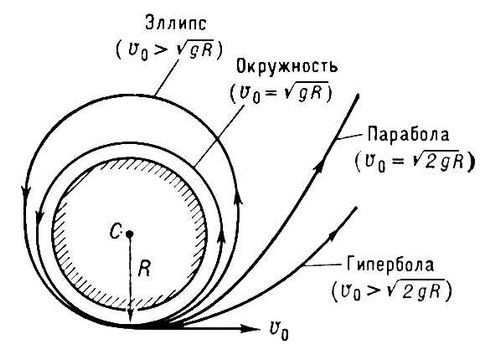
\includegraphics[width = 0.5\textwidth]{Space-speed}
\caption{Возможные траектории тела \label{pic:orbits}}
\end{figure}